\documentclass[11pt]{article}

% --- Packages ---
\usepackage[margin=1in]{geometry}
\usepackage{iftex}
\ifPDFTeX
  \usepackage[T1]{fontenc}
  \usepackage{lmodern}
\else
  \usepackage{fontspec}
  \setmainfont{DejaVu Serif}
\fi
\usepackage{microtype}
\usepackage{graphicx}
\usepackage{booktabs}
\usepackage{amsmath}
\usepackage{siunitx}
\usepackage{enumitem}
\usepackage[ruled,vlined,linesnumbered]{algorithm2e}
\DontPrintSemicolon
\SetKwInput{KwRequire}{Require}
\SetKwInput{KwReturn}{Return}
\usepackage[authoryear,round]{natbib}
\usepackage{hyperref}

% --- Hyperref setup ---
\hypersetup{
  colorlinks=true,
  linkcolor=blue,
  citecolor=blue,
  urlcolor=blue
}

% --- Convenience macros ---
\newcommand{\cmap}{Simons CMAP}
\newcommand{\cmapagent}{CMAP Agent}

% --- Vignette formatting ---
\newenvironment{vignettebox}{\begin{quote}\small}{\end{quote}}
\newcommand{\vignettefield}[2]{\textbf{#1:} #2\\}

\title{Agentic Retrieval-Augmented Interface for Natural-Language Data Discovery and Analysis in Environmental Sciences}
%\author{Mohammad D. Ashkezari \and \textit{(co-authors TBD)}}
\date{\today}

\begin{document}
\maketitle

\begin{abstract}
\cmapagent\ is an agentic, retrieval-augmented interface for interacting with the \cmap\ harmonized ocean (and atmospheric) data system.
The system enables users to express scientific intent in natural language and obtain verifiable results through a combination of
(i) semantic retrieval over a knowledge base derived from \cmap\ catalog metadata and documentation,
(ii) tool-based execution for dataset discovery, data subsetting, visualization, climatology, and dataset colocalization, and
(iii) optional emission of reproducible analysis code in the CMAP software ecosystem.
The contribution is a practical, domain-oriented agent design that couples LLM-driven planning with validated scientific tools and artifact-centric outputs,
reducing the barrier from question to executable analysis while supporting provenance and reproducibility.
Representative workflows and an evaluation framework are outlined for marine and environmental-science use cases.

\end{abstract}

\section{Introduction}
Marine and environmental research increasingly relies on integrating heterogeneous observations and model products across space and time.
Even when powerful data portals and programmatic APIs exist, the ``last-mile'' barrier often remains: scientists must discover appropriate datasets,
resolve identifiers, construct queries, and assemble analyses across multiple systems.

\cmap\ was designed to reduce these barriers by harmonizing diverse datasets into a common data and metadata structure and indexing entries by location and time,
enabling streamlined retrieval, visualization, and systematic data integration \citep{Ashkezari2021SimonsCMAP}.

An enabling condition for agentic analysis is that \cmap\ is a curated platform: datasets and metadata are vetted and harmonized by domain scientists, with stable identifiers and standardized descriptors.
This allows \cmapagent\ to use retrieval and tool execution as mechanisms for grounding---resolving scientific intent to catalog-backed dataset/variable definitions and producing verifiable artifacts---rather than relying on a model's latent knowledge alone.
However, effective use of a large harmonized catalog still requires users to translate scientific intent into specific catalog operations, parameter choices, and analysis workflows.

Recent advances in retrieval augmentation and tool-augmented LLM agents suggest a complementary approach:
retrieval-augmented generation improves grounding via explicit, updateable memory \citep{Lewis2020RAG},
while reasoning--acting loops enable verifiable computation through external tools \citep{Yao2022ReAct,Karpas2022MRKL}.
This article focuses on \cmapagent, an agentic layer built to support common CMAP workflows through a natural-language interface that executes validated operations and produces scientific artifacts.

\paragraph{Contributions.}
The paper emphasizes contributions specific to the agentic system (not the underlying \cmap\ portal):
\begin{enumerate}[leftmargin=*]
  \item A domain-oriented architecture for grounded, tool-augmented analysis of ocean and environmental data, integrating semantic catalog retrieval with validated computational tools.
  \item A capability suite that operationalizes common CMAP workflows (dataset discovery, spatiotemporal subsetting, visualization, and colocalization) with artifact-centric outputs.
  \item A reproducibility model that combines provenance records, downloadable artifacts, and optional executable SDK code to bridge conversational exploration and scripted analysis.
  \item An evaluation plan aligned with emerging benchmarks for tool-using and data analysis agents \citep{Zhang2024DSEval,Li2025IDABench}.
\end{enumerate}

\paragraph{Paper organization.}
Section~2 summarizes the \cmap\ data layer at a level sufficient to motivate the agentic interface.
Sections~3--7 position the system relative to prior work and describe the knowledge base, tool layer, and interaction model.
Sections~8--10 present representative workflows, an evaluation plan, and a discussion of limitations and future directions.


\section{Background: Simons CMAP as a Harmonized Earth-System Data Layer}
This section briefly characterizes the \cmap\ data layer at the level needed to contextualize the agentic system; a fuller account of the underlying portal is given in \citet{Ashkezari2021SimonsCMAP}.
\cmap\ harmonizes heterogeneous datasets into a common structure and indexes entries by location and time, enabling efficient retrieval and integration. The system exposes these capabilities via interactive and programmatic interfaces.

\paragraph{Curation and harmonization as a substrate for agents.}
CMAP is assembled through domain-scientist curation: ingest and documentation practices standardize metadata, references, and variable semantics across heterogeneous sources.
For an agentic interface, this curated substrate has two concrete consequences.
First, retrieval can anchor decisions in vetted descriptors---units, spatial and temporal coverage, instrument or model provenance---so that the agent's choice of a dataset or variable is grounded in catalog facts rather than inferred from the model's latent knowledge.
Second, tools can operate on consistent identifiers (table and variable short names) without per-dataset special cases, which is what makes a single, generic execution layer practical across hundreds of products.
We therefore treat the curated layer as a scientific enabler of reliable discovery and integration, not merely as an implementation convenience.


\section{Related Work}
The introduction has already named the foundational threads on which \cmapagent\ rests; this section situates those threads within the broader landscape and identifies the converging research directions on which the system's design draws.

\subsection{Retrieval augmentation, tool use, and grounded LLM agents}
Two complementary mechanisms have emerged for grounding large language models in external resources.
Retrieval-augmented generation (RAG) couples parametric language models with an explicit, updateable external memory, improving factuality and enabling provenance in knowledge-intensive settings \citep{Lewis2020RAG}; in scientific contexts, agentic variants iterate retrieval and synthesis across full-text papers and have been shown to match or exceed expert performance on literature-research tasks \citep{Lala2023PaperQA,Skarlinski2024PaperQA2}.
Tool augmentation extends this grounding from memory to action: ReAct interleaves reasoning and acting, demonstrating benefits for interpretability and reduced hallucination when models can query external resources \citep{Yao2022ReAct}; Toolformer shows that models can learn when and how to invoke tools through self-supervision \citep{Schick2023Toolformer}; and modular neuro-symbolic architectures such as MRKL argue for combining large language components with specialized reasoning and knowledge modules \citep{Karpas2022MRKL}.
\cmapagent\ draws on both threads: the knowledge base provides updateable retrieval-based grounding, while an explicit tool layer turns retrieved context into validated, executable operations.

\subsection{Scientific domain agents and their evaluation}
Recent systems demonstrate the scientific potential of tool-augmented LLM agents across domains.
ChemCrow integrates expert tools for chemistry and reports multi-step task success across synthesis and discovery workflows \citep{Bran2024ChemCrow}, and Coscientist demonstrates an agentic system that combines planning, tool use, and execution to carry out multi-step experimental procedures in an automated laboratory setting \citep{Boiko2023Coscientist}.
In ocean science, domain-focused models such as OceanGPT aim to improve performance on oceanography tasks via instruction data and domain benchmarks \citep{Bi2023OceanGPT}; in the geospatial domain, GeoGPT exemplifies an autonomous workflow paradigm in which a language model plans and executes GIS tools sequentially to complete user-specified geospatial tasks \citep{Zhang2024GeoGPT}; and beyond single-agent systems, multi-agent frameworks have been proposed for hypothesis generation and scientific exploration, including graph- and knowledge-based approaches \citep{Ghafarollahi2024SciAgents}.
A complementary strategy improves domain knowledge through pretraining: domain-specific foundation models for geoscience and climate (e.g., K2 and ClimateGPT) often pair this with retrieval augmentation for factuality \citep{Deng2023K2,Thulke2024ClimateGPT}.
Recent reviews of AI for geoscience synthesize progress in large-scale models, physics-informed approaches, and geoscientific applications, while emphasizing data governance, uncertainty, and interpretability challenges \citep{Zhao2024AIforGeoscience}; agentic RAG systems for environmental data can be viewed as one response to these challenges, grounding domain language in curated metadata, routing computations through validated tools, and returning artifacts that support auditability.
Reliable evaluation of such systems remains difficult because they must plan, act, recover from errors, and manage multi-step interactions: general-purpose agent benchmarks have been proposed for interactive environments \citep{Liu2023AgentBench}; tool-oriented benchmarks such as ToolBench (introduced alongside ToolLLM) and StableToolBench focus on large-scale evaluation of tool use and the stability of tool APIs \citep{Qin2023ToolLLM,Guo2024StableToolBench}; and for data analysis agents specifically, DSEval and IDA-Bench emphasize the end-to-end lifecycle and multi-round nature of practical analysis workflows \citep{Zhang2024DSEval,Li2025IDABench}.
These lines of work motivate \cmapagent\ as a domain-grounded, tool-executing assistant focused on scientific data discovery and analysis rather than model pretraining alone.

\subsection{Natural-language interfaces to scientific data}
Natural-language interfaces to structured data have a long history, and LLMs have renewed interest in text-to-SQL and database interfaces.
However, scientific workflows typically require more than query translation; they demand validation, iterative refinement, visualization, and the production of reusable analysis artifacts.
\cmapagent\ is positioned as an agentic layer that combines grounded catalog retrieval with domain tools and artifact-oriented outputs for ocean and environmental data analysis.


\section{System Overview}
Figure~\ref{fig:architecture} summarizes the \cmapagent\ architecture at the level of abstraction relevant to scientific users: retrieval over a domain knowledge base, agentic planning with tool-mediated execution, and artifact-oriented outputs with persisted provenance.

\begin{figure}[!ht]
  \centering
  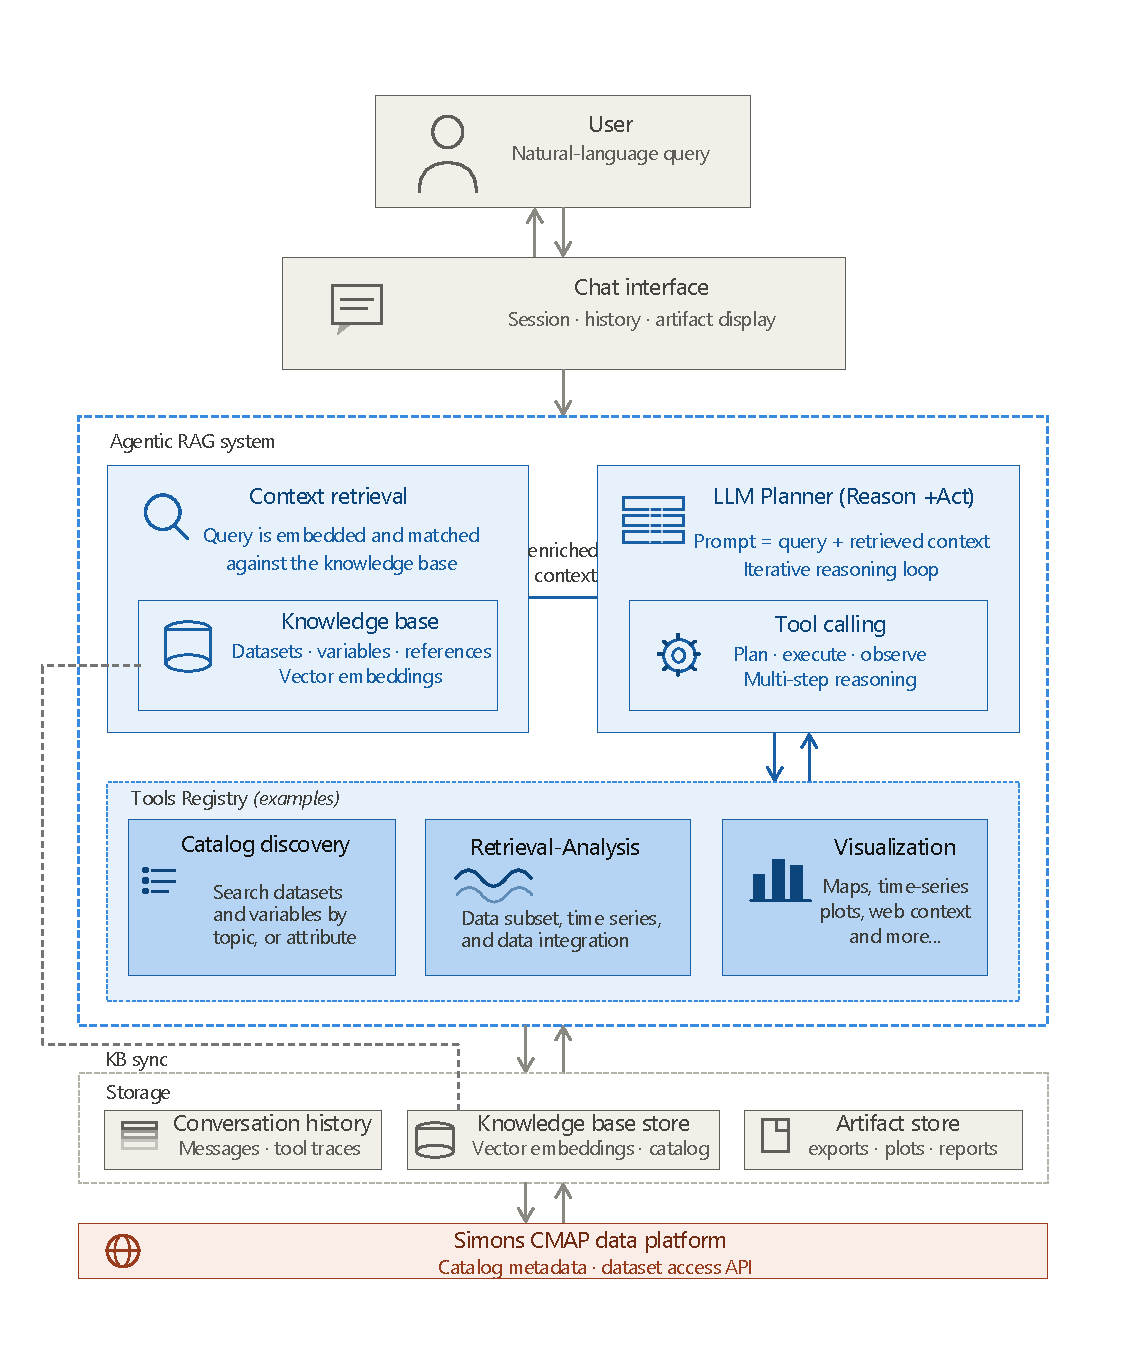
\includegraphics[width=\linewidth,height=0.6\textheight,keepaspectratio]{figures/architecture.pdf}
  \caption{Conceptual architecture of the conversational \cmapagent. User queries are processed through a Retrieval-Augmented Generation (RAG) pipeline that semantically searches a domain knowledge base---populated from the \cmap\ catalog---to enrich the prompt supplied to a foundation model. The model operates in an agentic loop, iteratively invoking specialized tools for dataset discovery, data retrieval, analysis, and visualization until a final response is synthesized. Conversation history, embeddings, and output artifacts are persisted across sessions, and the knowledge base is refreshed as the CMAP catalog evolves.}
  \label{fig:architecture}
\end{figure}

\paragraph{From intent to executable analysis.}
The system is designed to translate open-ended scientific intent (e.g., ``compare chlorophyll and SST seasonality in a region'') into a sequence of verifiable operations:
dataset/variable resolution, spatiotemporal subsetting, optional integration of multiple datasets, computation, and visualization.
Rather than asking users to learn internal catalog identifiers and calling conventions, the agent performs these steps while exposing intermediate decisions through tool traces and returned artifacts.

\paragraph{Grounding and verifiability.}
Two mechanisms are central.
First, retrieval over a curated knowledge base provides domain context (catalog entries, variable semantics, and usage guidance) to reduce hallucination and improve correct dataset selection.
Second, analyses are executed through explicit tools with constrained inputs and programmatic validation, so that computations and figures are produced by deterministic routines rather than free-form text.

\paragraph{Artifact-oriented outputs and reproducibility.}
Outputs are centered on scientific artifacts: subsets of data, figures, and (when appropriate) reusable code snippets that reproduce the same operations in the CMAP software ecosystem.
This design supports interactive exploration while enabling transition to scripted workflows for publication-quality analyses.

\paragraph{Separation of scientific semantics from implementation.}
While the system is realized as a concrete software stack, the scientific claims in this paper emphasize capability and behavior rather than the specifics of frameworks or deployment.
This separation is important for long-lived scientific infrastructure, where engineering choices may evolve while the user-facing semantics and provenance guarantees remain stable.


\section{Knowledge Base and Retrieval}
\subsection{Scope and grounding in dataset literature}
The knowledge base is constructed from \cmap\ catalog descriptors and supporting materials---dataset references, variable lists, and curated help content---and is augmented with full-text scientific documents associated with individual datasets.
This composition supports two complementary goals: reliable resolution of datasets, variables, and operational constraints (e.g., valid ranges in depth and time), and access to methodological detail that is often absent from catalog metadata (e.g., sampling protocols, calibration procedures, and quality-control criteria).
Beyond catalog descriptors, many scientifically consequential facts are documented only in the literature that accompanies a dataset, and to make these facts retrievable the system ingests and indexes dataset-linked reference documents (papers, technical reports, and documentation) on a per-dataset basis.
This design enables questions about collection and processing methods, caveats, and recommended use conditions to be answered by retrieving passages from primary sources, while preserving an explicit link from each retrieved passage back to the dataset it documents.
By coupling a dataset-specific literature corpus to a curated data catalog, the approach extends literature-grounded question answering systems \citep{Lala2023PaperQA,Skarlinski2024PaperQA2} into a setting where retrieved evidence can immediately inform downstream, tool-executed analysis.

\begin{figure}[!ht]
  \centering
  \includegraphics[width=\linewidth]{figures/reference_bank.pdf}
  \caption{Grounding the agent in the literature behind each dataset. A catalog entry is documented by one or more references (publications, technical reports, methods manuals). These documents are extracted, segmented into chunks, and indexed alongside catalog descriptors in a shared knowledge base; each chunk carries an explicit back-pointer to the dataset it documents. A methodological question---one whose answer is contained in a paper rather than in catalog metadata---is then served by the same hybrid retrieval channel that surfaces catalog entries, returning both the passage and the identity of the dataset it documents.}
  \label{fig:refbank}
\end{figure}

\subsection{Retrieval and planning}
Scientific methods and protocols are frequently expressed in specialized vocabulary and in numerically specific statements.
To reduce failure modes in which semantically similar but technically irrelevant passages dominate retrieval, the knowledge base supports retrieval that combines semantic similarity with lexical matching for identifiers, numbers, and exact terms; ranked lists from these complementary signals can be fused using standard rank-fusion approaches \citep{Bruch2023FusionFunctions}, improving robustness without requiring per-query tuning or assuming a single representation is sufficient for all query types.
At each interaction turn, the resulting compact set of knowledge snippets is supplied to the agent and used to condition its planning, following the central RAG principle of coupling generation to an explicit, updateable memory in order to improve factuality and traceability \citep{Lewis2020RAG}.
In \cmapagent, this conditioning serves not only descriptive responses (e.g., catalog interpretation) but also reduces error rates in tool selection and parameterization---for example, resolving the intended dataset table and variable before subsetting, visualization, or colocalization.

\subsection{Refreshability and reproducibility}
Because catalogs and their associated literature evolve, the knowledge base is designed to be refreshable: catalog descriptors can be re-synchronized and reference corpora can be augmented as new documentation becomes available, without retraining the language model.
When retrieval is used, the agent can summarize or cite retrieved snippets to clarify why a dataset, variable, or processing choice was made.
Outputs are returned as persistent artifacts---figures, data exports, and, where appropriate, executable code---that capture the operations performed at the time of the analysis; combined with the refreshability of the knowledge base, this allows an analysis to be re-executed against a later state of the catalog so that any change in its output is attributable to the underlying data rather than to the agent.


\section{Tooling and Execution}
A central design goal is that scientific operations are executed through explicit computational tools, while the language model focuses on translating intent into a validated sequence of actions.
This aligns with research on tool-augmented agents, where external actions provide verifiable intermediate results and reduce reliance on unconstrained text generation \citep{Yao2022ReAct,Karpas2022MRKL}.

\subsection{Capability categories}
The tool layer operationalizes common workflows in ocean and environmental data analysis:
\begin{itemize}[leftmargin=*]
  \item \textbf{Discovery and resolution:} identify candidate datasets and variables, interpret metadata, and disambiguate naming.
  \item \textbf{Data access:} retrieve spatiotemporal subsets with user-defined bounds and sampling options.
  \item \textbf{Analysis:} compute derived products such as climatologies and summary statistics.
  \item \textbf{Integration:} colocalize datasets by joining observations and gridded products within spatial/temporal tolerances.
  \item \textbf{Visualization:} generate quick-look figures (maps, time series) that summarize retrieved subsets.
  \item \textbf{Reproducible code:} optionally emit executable code that reproduces the same operations in the CMAP SDK.
\end{itemize}

\subsection{Representative tool outputs}
Many interactions produce both a narrative response and scientific artifacts (data files, figures).
Table~\ref{tab:capabilities} summarizes the primary capability classes and expected outputs.

\begin{table}[h]
\centering
\small
\begin{tabular}{@{}p{0.34\linewidth}p{0.61\linewidth}@{}}
\toprule
\textbf{Capability} & \textbf{Typical outputs} \\
\midrule
Catalog discovery and variable resolution & Candidate datasets/variables with brief justification grounded in catalog context \\
Spatiotemporal subsetting & Downloadable data subset (e.g., Parquet/CSV) with provenance notes \\
Quick-look visualization & Map plots or time-series figures derived from retrieved subsets \\
Climatology and summaries & Climatology fields or seasonal cycles; summary tables/figures \\
Colocalization / dataset integration & Joined tables for multi-dataset analysis; tolerance settings and diagnostics \\
Code emission (optional) & Executable SDK code reproducing the performed operations \\
\bottomrule
\end{tabular}
\caption{Capability-oriented summary of \cmapagent. The underlying implementation exposes these functions through structured tool contracts; the main text emphasizes scientific functionality rather than specific software frameworks.}
\label{tab:capabilities}
\end{table}

\subsection{Iterative planning and tool execution loop}
At the core of \cmapagent\ is a per-turn runner that alternates between (i) requesting a structured plan from the language model and (ii) executing the requested tool calls.
The runner enforces a strict JSON protocol with two message types: \texttt{tool\_call} (a list of tool invocations) and \texttt{final} (the user-facing response).
It also implements practical guardrails that matter for scientific use: a configurable tool-call budget, caching of identical tool calls to avoid accidental loops, sanitization of co-localization tolerances when they were not specified by the user, and aggregation of tool-produced artifacts (e.g., plots and data extracts) into the final response.
Algorithm~\ref{alg:execute_plan} summarizes this control flow in compact pseudocode format.

\begin{algorithm}[!ht]
\caption{Per-turn agent runner (conceptual) implementing an iterative plan--execute--observe loop with key guardrails: strict structured outputs, bounded tool usage, per-turn deduplication, co-localization tolerance sanitization, and aggregation of tool-produced artifacts and optional reproducible code into the final response.}
\label{alg:execute_plan}
\small
\SetAlgoNlRelativeSize{-1}
\DontPrintSemicolon
\KwRequire{system prompt; conversation history; user message; execution context; tool-call budget $B$}
\KwResult{final response (message + optional code + artifact references), and tool trace for provenance}

$M \leftarrow [\textsf{SYSTEM}(\texttt{system\_prompt})] + \textsf{conversation} + [\textsf{USER}(\texttt{user\_message})]$\;
$T \leftarrow [\ ]$; $A \leftarrow [\ ]$; $C \leftarrow [\ ]$; $\mathcal{H} \leftarrow \emptyset$ \tcp*[r]{trace, artifacts, code, dedup cache}\;
$b \leftarrow \max(0,B)$; $r_{\textsf{json}}\leftarrow 0$; $r_{\textsf{force}}\leftarrow 0$\;
\If{$b = 0$}{Append to $M$ an instruction that tools are disabled and the planner must return \texttt{final}.}\;

\Repeat{a \texttt{final} response is produced}{
  $\texttt{resp} \leftarrow \textsc{LLMComplete}(M)$\;
  \If{\textsc{StrictJSONWithType}(\texttt{resp}) is false}{
    \If{$r_{\textsf{json}}<2$}{
      $r_{\textsf{json}}\leftarrow r_{\textsf{json}}+1$; Append a JSON-only repair instruction to $M$; \textbf{continue}\;
    }
    \KwRet{\textsc{FinalizeFromText}(\texttt{resp},A,C), $T$}\;
  }

  $(\texttt{kind},\texttt{payload}) \leftarrow \textsc{ParsePlanOrFinal}(\texttt{resp})$\;
  \If{$\texttt{kind}=\texttt{final}$}{
    $\texttt{final} \leftarrow \textsc{ValidateOrStringify}(\texttt{payload})$; merge $A$ and (optionally) $C$ into \texttt{final}\;
    \If{\textsc{RequestRequiresTools}(\texttt{user\_message}) and $T$ is empty and $b>0$ and $r_{\textsf{force}}<2$}{
      $r_{\textsf{force}}\leftarrow r_{\textsf{force}}+1$; append an instruction forcing a \texttt{tool\_call} response to $M$; \textbf{continue}\;
    }
    \KwRet{\texttt{final}, $T$}\;
  }
  \If{$\texttt{kind}\neq\texttt{tool\_call}$ or $b=0$}{Append to $M$ an instruction to return \texttt{final}; \textbf{continue}}\;

  $R \leftarrow [\ ]$ \tcp*[r]{compact results for planner}\;
  \ForEach{requested tool call $(\tau,\alpha)$ \textbf{while} $b>0$}{
    \If{$\tau=\texttt{cmap.colocalize}$}{$\alpha \leftarrow \textsc{SanitizeColocalizeArgs}(\texttt{user\_message},\alpha)$}\;
    $k \leftarrow (\tau,\textsc{CanonicalArgs}(\alpha))$\;
    \uIf{$k \in \mathcal{H}$}{
      $\texttt{compact} \leftarrow \mathcal{H}[k]$; record \texttt{cached} in $T$\;
    }
    \Else{
      $\texttt{result} \leftarrow \textsc{RunTool}(\tau,\alpha,\texttt{exec\_context})$\;
      normalize artifacts into $A$; append any emitted SDK code into $C$\;
      $\texttt{compact} \leftarrow \textsc{SummarizeForPlanner}(\tau,\texttt{result})$; set $\mathcal{H}[k]\leftarrow\texttt{compact}$\;
      record status/errors in $T$; $b\leftarrow b-1$\;
    }
    Append \texttt{compact} to $R$\;
  }
  Append a compact \texttt{TOOL\_RESULTS} observation containing $R$ to $M$\;
}
\end{algorithm}

\subsection{Validation and failure modes}
Inputs to computational tools are validated (e.g., numeric bounds, required parameters, tolerance ranges), and intermediate failures can be surfaced to the user with actionable messages.
This design supports iterative refinement, which is characteristic of real-world analysis and is emphasized by recent evaluations of data analysis agents \citep{Zhang2024DSEval,Li2025IDABench}.


\section{User Interface and Interaction Model}
\paragraph{Interaction model.}
The user-facing interface supports conversational sessions with persistent thread history.
Within a session, requests may alternate between high-level scientific questions (``what data are available for mixed-layer depth?'') and procedural instructions (``plot a time series in this region and period'').
Responses may include explanatory text, generated figures, downloadable data subsets, and optional executable code.

\paragraph{Artifact presentation.}
Artifacts are treated as first-class outputs.
Figures can be previewed inline, while data subsets are offered as downloadable files suitable for direct use in notebooks or scripts.
This presentation helps bridge exploratory dialogue with reproducible analysis workflows.

\paragraph{Traceability.}
When tool-based operations are executed, provenance information (e.g., selected datasets/variables, bounds, and processing steps) can be summarized alongside results.
In practice, the interface can present this provenance as an optional, compact view (e.g., an expandable tool trace that can be copied or archived).
Such traces are important for scientific credibility and for debugging multi-step requests, consistent with broader calls for grounded, interpretable agent trajectories \citep{Yao2022ReAct}.


\section{Representative Workflows and Applications}
This section presents representative workflows that reflect common ocean and environmental science tasks.
The intent is not to prescribe a single ``best'' analysis path, but to illustrate how the \cmapagent\ (Fig.~\ref{fig:architecture}) turns natural-language intent into grounded, tool-executed operations with artifact-oriented outputs.
Across workflows, the agent (i) resolves datasets and variables using catalog-grounded context, (ii) executes validated operations through tools rather than free-form text, and (iii) returns persistent artifacts (data files, figures, and optional executable SDK code) to support reproducibility.

\subsection{Workflow 1: Concept-driven discovery and bounded data extraction}
Many sessions start with a scientific concept rather than a known table name.
For example, a user may ask for ``satellite chlorophyll concentration over the North Pacific Ocean'' or request candidate datasets for ``mixed-layer depth''.
The workflow proceeds in three stages:
\begin{enumerate}[leftmargin=*]
  \item \textbf{Concept-to-catalog grounding.} The agent retrieves relevant catalog context (dataset descriptions, variable lists, references) and proposes a small set of candidate datasets/variables.
  \item \textbf{Interactive disambiguation.} When multiple plausible candidates exist, the agent asks targeted follow-up questions (e.g., desired resolution, in-situ vs. gridded) to ensure the intended product is selected.
  \item \textbf{Bounded extraction as an artifact.} Once selected, the agent executes a spatiotemporal subset request and returns a downloadable artifact (e.g., CSV/Parquet) along with the bounds used and optional SDK code to reproduce the query.
\end{enumerate}
This pattern mirrors how scientists typically explore a portal: search, compare candidates, then extract a bounded subset for downstream analysis.
The key difference is that the interface is intent-first and grounded in the catalog, reducing the need for users to know internal identifiers up front.

\subsection{Workflow 2: Rapid visualization and climatological summaries}
Exploratory visualization is often the fastest way to validate whether a chosen dataset matches a hypothesis.
In \cmapagent, visualization requests are expressed at the level of scientific intent (map vs. time series; region vs. point; time range), and executed through deterministic plotting routines.
Two recurring patterns are:
\begin{enumerate}[leftmargin=*]
  \item \textbf{Quick-look plots from extracted subsets.} The agent produces maps or time series from a retrieved subset and returns the figure as an artifact, enabling immediate inspection and iteration.
  \item \textbf{Climatology and seasonal-cycle summaries.} For gridded products, users commonly request climatological means or seasonal cycles (e.g., ``mean monthly SST'' or ``seasonal chlorophyll'').
  The agent executes the corresponding aggregation, returns the derived dataset as an artifact, and generates a diagnostic plot that summarizes the seasonal structure.
\end{enumerate}
These outputs help users validate assumptions early (e.g., coverage, units, expected seasonality) before committing to larger analyses.
They also provide a bridge from conversational exploration to publication workflows by returning reusable artifacts and, optionally, executable code.

\subsection{Workflow 3: Dataset integration by colocalization}
Ocean science frequently requires integrating sparse in-situ observations with gridded satellite or model products.
CMAP provides a harmonized spatiotemporal index that supports this operation at scale \citep{Ashkezari2021SimonsCMAP}; \cmapagent\ makes the integration accessible through intent-level instructions.
In a typical colocalization workflow:
\begin{enumerate}[leftmargin=*]
  \item \textbf{Source selection.} The user specifies a source table (e.g., in-situ observations) and one or more target products (e.g., satellite SST), or provides a user-owned dataset as an uploaded artifact.
  \item \textbf{Tolerance specification.} The agent confirms spatial/temporal tolerances (and, where relevant, vertical matching assumptions) and validates that tolerances are within supported ranges.
  \item \textbf{Join execution and diagnostics.} The agent executes the join and returns an integrated table artifact, along with summary diagnostics (e.g., match counts, bounds used) and optional code for reuse.
\end{enumerate}
By returning the joined dataset as a file, the workflow supports downstream modeling, statistical analysis, and reproducible figure generation.
More broadly, it illustrates the core scientific promise of agentic interfaces: enabling multi-step, verifiable data operations without requiring users to manually orchestrate every intermediate command.

\subsection{Reporting provenance to support scientific trust}
Across workflows, the system can surface concise provenance: which dataset/variable candidates were considered, what bounds and tolerances were applied, and what artifacts were produced.
This emphasis on traceable, tool-executed trajectories aligns with broader findings in agent research that interleaving reasoning with actions can improve interpretability and reduce unsupported generation \citep{Yao2022ReAct}.
In \cmapagent, provenance also serves a practical purpose: it allows users to copy results into notebooks, share analyses with collaborators, and audit results when preparing figures for publication.


\subsection{Session vignettes with artifacts and provenance}
To avoid synthetic demonstrations, the paper will include short vignettes drawn from real \cmapagent\ sessions.
Each vignette reports (i) the user prompt, (ii) a compact provenance snippet summarizing tool calls and key parameters, and (iii) the resulting artifacts (e.g., tabular extracts and figures) suitable for direct reuse in notebooks.
The vignettes are intentionally brief and are meant to complement, not replace, the higher-level workflow descriptions above.

%\subsubsection*{Vignette 1: Concept-driven discovery and bounded extraction}
\begin{vignettebox}
\vignetteprompt{\textit{(User prompt)}}
\vignettefield{Condensed provenance}{\textit{(a compact tool-trace summary: tool names, key bounds/tolerances, and any dataset/variable resolutions.)}}
\vignettefield{Artifacts}{\textit{(List artifacts)}}
\end{vignettebox}


\subsubsection*{Vignette 1: Catalog discovery and visualization}
\begin{vignettebox}
\vignettefield{Prompt}{\textit{Make a Robinson-projected global map of total cloud cover in December 1945. Use an appropriate dataset available in CMAP and return the plot as an image.}}
\vignettefield{Condensed provenance}{Tools: Search Knowledge base, Plot map}
\vignettefield{Artifacts}{Python code to extract data, Download link to data, Generated visualization Fig.~\ref{fig:vin_viz}. }
\end{vignettebox}



\begin{figure}[t]
  \centering
  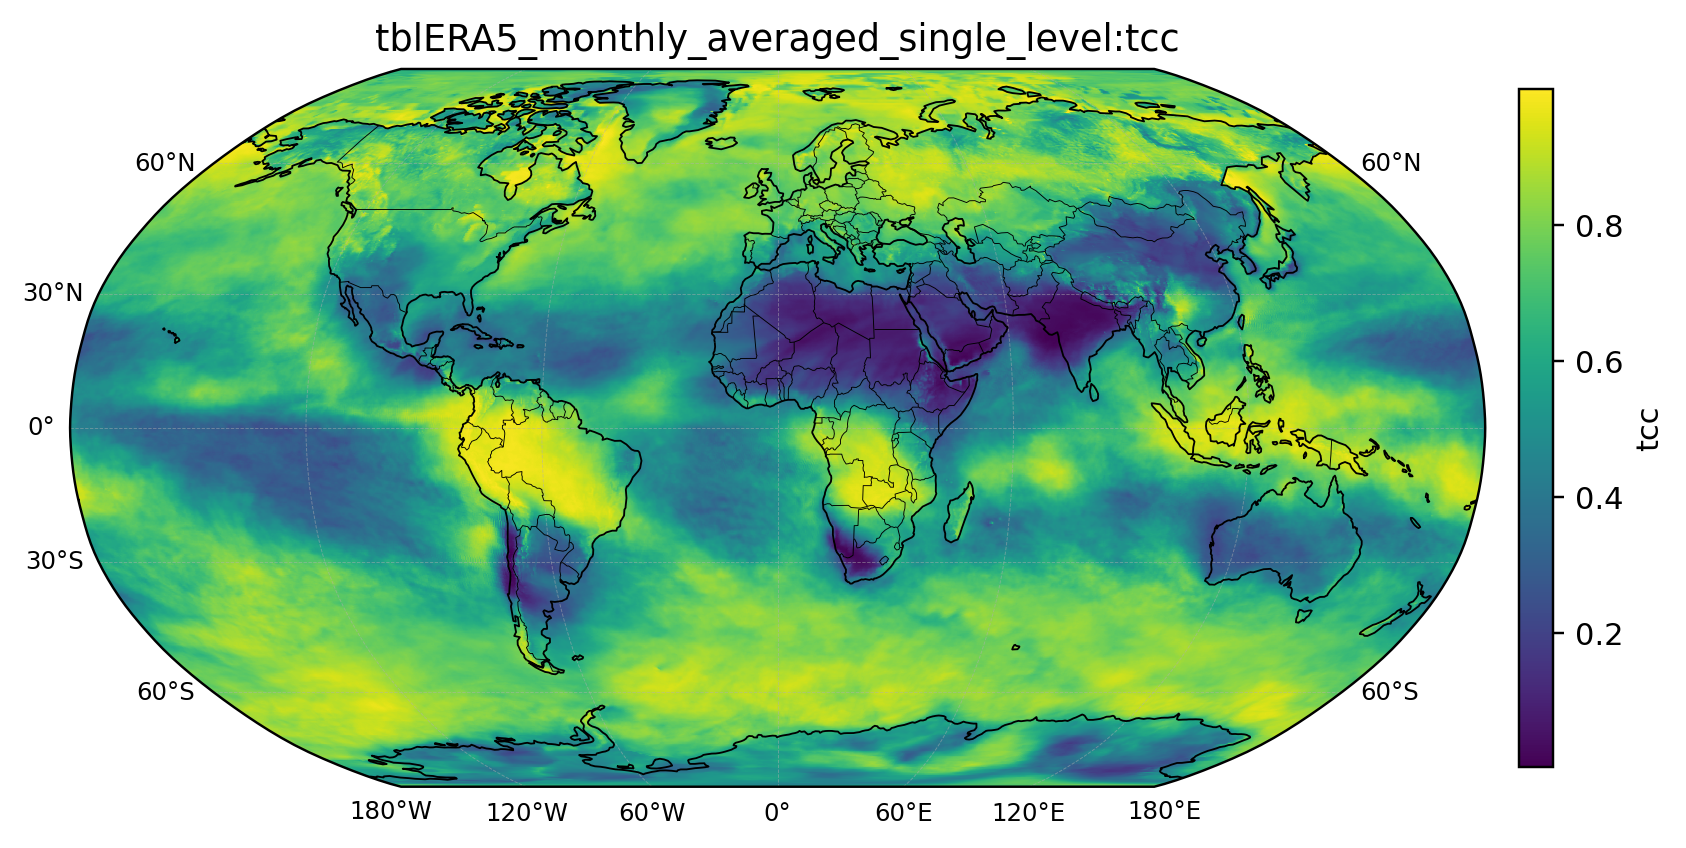
\includegraphics[width=\linewidth]{figures/tcc.png}
  \caption{Visualization workflow vignette. From a natural-language request, CMAP Agent generates a global map visualization of total cloud cover (tcc) for December 1945 from the ERA5 Monthly Averaged Single Levels dataset. Colors indicate cloud fraction, with coastlines and political boundaries overlaid for geographic context. The figure illustrates the agent’s ability to resolve a dataset/variable, retrieve the required subset, and produce a georeferenced map artifact that is returned as a downloadable figure file in a standard cartographic projection (Robinson)}
  \label{fig:vin_viz}
\end{figure}

\subsubsection*{Vignette 2: Dataset integration via co-localization}
\begin{vignettebox}
\vignettefield{Prompt}{\textit{Can you colocalize the 'Discrete Flow Cytometry of Underway Samples from TN427 Using a BD Influx Cell Sorter' dataset with: 
total precipitation (tp in tblERA5\_monthly\_averaged\_single\_level) from ERA5 dataset, 
and daily satellite SST (sst in tblSST\_AVHRR\_OI\_NRT), 
and Nitrate monthly climatology from the World Ocean Atlas 2013 v2 Climatology dataset (nitrate\_WOA\_clim in tblWOA\_Climatology)?}}
\vignettefield{Condensed provenance}{Tools: catalog search and colocalization}
\vignettefield{Artifacts}{python code for colocalization and the final integrated dataset is returned.}
\end{vignettebox}


\section{Evaluation Plan}
Evaluation is framed around scientific utility and operational reliability rather than conversational quality alone.
This aligns with recent calls to evaluate agents across multi-step lifecycles and interactive analysis settings \citep{Zhang2024DSEval,Li2025IDABench}.

\paragraph{Current internal retrieval evaluation.}
A first evaluation has been performed at the level of the retrieval substrate, which provides the grounding evidence used both for question answering and for tool selection.
In an initial study ($N=108$) of reference-grounded queries whose answers are known to exist in the indexed corpus, the correct evidence passage is retrieved within the top-$32$ results in $95.4\%$ of cases, with median rank $1$.
These results should be interpreted as a preliminary characterization of retrieval robustness for technically specific facts (e.g., numeric thresholds and protocol details), rather than as an end-to-end assessment of the full agent.
A comprehensive evaluation that exercises the complete plan--execute--observe loop (including dataset/variable resolution, parameterization, and artifact production), curated and reviewed by domain scientists, is in preparation.

\paragraph{Benchmark prompt suite.}
A curated suite of prompts will cover: dataset discovery, variable resolution, spatiotemporal subsetting, visualization, climatology, and colocalization.
The suite can be seeded from maintained example prompts (included as supplementary material) and extended with domain-expert authored tasks.

\paragraph{Potential Metrics.}
\begin{itemize}[leftmargin=*]
  \item \textbf{Resolution correctness:} selection of the intended dataset table(s) and variable(s), judged against expert labels.
  \item \textbf{Tool success rate:} fraction of tasks completed without execution errors, including appropriate recovery on the first retry.
  \item \textbf{Output validity:} basic sanity checks on returned artifacts (e.g., non-empty subsets; expected dimensions; figure generation success).
  \item \textbf{Reproducibility:} ability to reproduce artifacts from emitted code or logged parameters.
  \item \textbf{Efficiency:} number of tool calls and end-to-end latency distributions (descriptive).
\end{itemize}

\paragraph{Baselines and comparisons.}
Comparisons may include: (i) direct use of the CMAP SDK without agent assistance, and (ii) ``chat-only'' LLM baselines without tool execution.
Where relevant, evaluation protocols can draw on broader agent benchmarks that emphasize interactive decision making \citep{Liu2023AgentBench} and tool-use performance \citep{Qin2023ToolLLM,Guo2024StableToolBench}.


\section{Discussion and Limitations}
\paragraph{Scientific value.}
The primary scientific value of an agentic interface is the reduction of ``activation energy'' from intent to executable analysis.
In practice, many ocean and environmental workflows begin with an under-specified concept (e.g., ``surface chlorophyll''), evolve through interactive refinement (time window, region, depth), and culminate in artifacts (subsets, figures, joined datasets) that are used in notebooks and publications.
\cmapagent\ is designed to support this lifecycle by grounding intent in catalog context, routing computation through validated tools, and returning artifacts with concise provenance.

\paragraph{Why a curated data layer matters.}
Many proposed scientific agents assume access to high-quality external resources (databases, tools, laboratory interfaces, or full-text corpora) and emphasize verifiable execution over free-form generation \citep{Bran2024ChemCrow,Boiko2023Coscientist,Lala2023PaperQA}.
In the ocean and environmental setting, a harmonized and curated catalog provides an analogous substrate: it reduces ambiguity in dataset/variable resolution and improves the reliability of tool-mediated operations.

\paragraph{Limitations and failure modes.}
Several limitations remain that are common to tool-using agents.
First, ambiguous scientific language can lead to incorrect dataset/variable resolution, particularly when multiple products exist with similar semantics.
Second, retrieval quality depends on the completeness and precision of catalog metadata and supporting documentation.
Third, complex analyses often require methodological choices (filters, statistical models, uncertainty quantification) that should be made explicitly by users rather than inferred implicitly.
Finally, multi-step planning can fail due to compounding errors, highlighting the need for structured self-correction and robust evaluation protocols for interactive workflows \citep{Liu2023AgentBench,Zhang2024DSEval}.

\paragraph{Trust, governance, and scientific accountability.}
Scientific assistants must address provenance, reproducibility, and data governance.
Tool traces and artifact-based outputs provide a foundation for transparency, consistent with the broader argument that interleaving reasoning with actions yields more interpretable trajectories \citep{Yao2022ReAct}.
However, stronger mechanisms are still needed: citation-style attribution for retrieved knowledge, guardrails for costly queries, and explicit uncertainty reporting.
Experience from scientific agents in other domains underscores the importance of verifiable execution and careful scoping (e.g., chemistry agents that integrate tools and execution environments) \citep{Bran2024ChemCrow,Boiko2023Coscientist}.

\paragraph{Future directions.}
Several research and development directions are motivated by both the agent literature \citep{Luo2025LLMAgentSurvey} and current needs in Earth-system data analysis \citep{Zhao2024AIforGeoscience}:
\begin{itemize}[leftmargin=*]
  \item \textbf{Richer scientific operations.} Expand uncertainty-aware and geospatial analysis routines (e.g., quality control diagnostics, comparability checks across products, and uncertainty propagation) so that common scientific workflows can be executed end-to-end with verifiable outputs.
  \item \textbf{Human-in-the-loop steering.} Make intermediate assumptions explicit and support structured user confirmation before expensive operations (e.g., choosing among multiple candidate products or tolerances). This is particularly important for ambiguous terminology and for workflows with many defensible methodological choices.
  \item \textbf{Citation-granular provenance.} Tighten the coupling between retrieved snippets and generated explanations so that users can audit where specific claims or dataset choices came from, complementing artifact-level provenance.
  \item \textbf{Cross-portal interoperability.} Extend retrieval and tool execution across multiple environmental data systems to support interdisciplinary workflows and reduce fragmentation.
  \item \textbf{Evaluation at scale.} Develop larger task suites and automated validity checks informed by emerging benchmarks for tool use and interactive analysis \citep{Qin2023ToolLLM,Guo2024StableToolBench,Zhang2024DSEval,Li2025IDABench}.
  \item \textbf{Domain model synergy.} Explore combinations of agentic tool execution with domain-tuned foundation models for geoscience and climate (e.g., K2, ClimateGPT) to improve terminology handling and reduce hallucinations, while preserving the verifiability benefits of tool-mediated computation \citep{Deng2023K2,Thulke2024ClimateGPT}.
\end{itemize}


\section{Conclusion}
\cmapagent\ demonstrates a practical agentic RAG architecture for scientific data systems, coupling semantic retrieval with explicit tool execution and artifact-centric outputs.
The system is designed to reduce the translation burden from scientific intent to executable data operations while preserving verifiability and reproducibility.

% TODO: Replace with a results-grounded conclusion once workflows and evaluation are completed.


\section*{Reproducibility and Availability}
The system comprises a server component (agent service and tool layer) and a web-based client interface.
Reproducibility is supported by (i) retaining tool parameters and intermediate outcomes as provenance records, (ii) returning downloadable artifacts alongside narrative explanations, and (iii) optionally emitting executable SDK code that reproduces performed operations.

For publication, an archival release (versioned source + container specifications) and a prompt suite used for evaluation can be provided.
Implementation details (e.g., frameworks, storage backends, and deployment configuration) are treated as engineering decisions and may evolve without changing the scientific capabilities described in this paper.


\paragraph{Vignette capture for publication.}\label{sec:reproducibility_vignettes}
The session vignettes in Section~8 are intended to be populated only from real system runs.
A recommended workflow is: (i) run the interaction in the web client; (ii) save the exact user prompt; (iii) export or copy the tool trace shown in the interface; and (iv) record the returned artifact identifiers (file names or persistent URLs).
The vignette templates under \texttt{supp/vignettes/} ensure that reported steps and outputs correspond exactly to recorded provenance.
No synthetic artifacts or fabricated tool traces are used.


\bibliographystyle{plainnat}
\bibliography{bib/references}

\end{document}
